% Created:  Fri 04 Jul 2014 04:47 PM
% Modified: Thu 31 Jul 2014 06:17 PM
% @author Josh Wainwright
% File name : imagej_plugin.tex

\section{ImageJ Plugin}
\label{sec:imagej_plugin}

% TODO section about the aims of the plugin etc.
\cite{imagejapi}

\subsection{Displaying the QuadTree}
\label{sub:displaying_the_quadtree}

The first version of the plugin simply allowed the user to visualise the data,
once it had been processed and entered into a quadtree. Though this provided
little benefit to the researcher producing data, it can be a useful tool to get
an insight into the process that a program is using to analyse one's data so
that the results can be better interpreted. For this reason, this version
served as a foundation for later versions of the plugin so that, when loading
data, a user gets the opportunity to view the data before proceeding with the
analysis.

Again, earlier versions of the program displayed this data using the built-in
GUI classes in the AWT\cite{zukowski1997java} and Swing\cite{loy2002java}
libraries included in the standard Java distribution. This effectively
prohibited any further actions being performed on the image once it had been
generated since what was displayed was only modifiable by the JVM via compiled
code. It was also very memory intensive since, in many cases, many thousands of
separate objects (data points represented by zero length lines, quadtree cells
by boxes, etc.) and so was slow to draw initially and redraw with any
subsequent move or resize of the window.

The code used to generate this view of the data was modified to make use of the
easy image generation functions present in ImageJ. Now, instead of many
different objects being manipulated for each view of the data, a single array
with a value for each pixel is needed. For the cases where the user wishes to
view the clusters that have been found, but not have them affect the image, the
image is created with a number of different \emph{slices} in the image
\emph{stack}, Figure~\ref{fig:imagej-stack}. Slices are ImageJ's representation
of images with two or more layers, or alternative views, each of which resides
in a stack of slices. Each slice in a stack must have the same dimensions.

\begin{figure}[tbhp]
	\centering
	\includegraphics[width=7cm]{imagej-stack.pdf}
	\caption{An ``image'' in ImageJ can be composed of a number of layers, each
		of which is easily viewable and can be saved on its own. These layers
		are used to display different parts of the generated image: data
		points, located clusters, quadtree structure, etc.}
	\label{fig:imagej-stack}
\end{figure}

\subsection{Column Picker}
\label{sub:column_picker}

% TODO writing about column picker

\subsection{Results Table}
\label{sub:results_table}

In addition to the image of the data with the clusters, the plugin also
calculates a number of statistics for each of the clusters that are found.
These include the number of points that are included in the cluster, the area
of the cluster, and it's perimeter. The area and perimeter values are given as
a fraction where the whole image represents 1. Thus, to find the actual area
for the real life object, the area of the cluster should be multiplied by the
area of the image, and for the perimeter, the length of one side of the image
should be multiplied by the perimeter.

To calculate each of these values, each node that exists in a cluster is
examined and its contribution to the overall value added.

\subsubsection{Cluster Area}
\label{ssub:Cluster Area}

To calculate the area of the clusters, each node in each cluster is examined.
Since the size of the node must be known, it is calculated from the quadtree
code for that node. The formula is shown in Equation~\ref{eq:node-area},
\begin{align}
	a &= \frac{1}{4^{d}} \\
	a_i &= 4^{-l_i/2}, \label{eq:node-area}
\end{align}
where $a_i$ is the area of the node $i$, $d$ is the depth in the quadtree and
$l_i$ is the length of the quadtree code of that node. For every node in the
cluster, where there are $n$ nodes, this value is summed to give the total
cluster area, $A$:
\begin{align}
	A &= \sum_{i=0}^{n} a_i.
\end{align}

\subsubsection{Cluster Perimeter}
\label{ssub:Cluster Perimeter}

Similarly to the cluster area, the perimeter is given as a fractional value of
the length of one side of the whole image, as calculated for each node from the
quadtree code, as shown in Equation~\ref{eq:node-perimeter},
\begin{align}
	p &= \frac{1}{2^{d}} \\
	p_i &= 2^{-l_i/2}, \label{eq:node-perimeter}
\end{align}
where the symbols have the same meaning as above.

However, this simply gives the length of one side of the node for any node. In
order to calculate the perimeter of the cluster, it is not enough to simply
sum these values, as for the cluster area, since not all nodes contribute to
the perimeter. Instead, for each node, it must be decided whether it
contributes to the perimeter and how much (1, 2, 3 or 4 sides), and then
increase the total perimeter by this many times the length of one side. The
total perimeter, $P$, then is given by Equation~\ref{eq:total-perimeter},
\begin{align}
	P &= \sum_{i=0}^{n} s * p_i, \label{eq:total-perimeter}
\end{align}
where $s \in \{0..4\}$. This is demonstrated in
Figure~\ref{fig:perimeter-edges} where the perimeter is simple to calculate in
case a) as the nodes are all the same, but the size of each node must be taken
into account in case b).

\begin{figure}[tbhp]
	\centering
	\begin{subfigure}[c]{3.5cm}
		\includegraphics[width=\textwidth]{perimeter-edges-grid.pdf}
		\caption{}\label{fig:perimeter-edges-grid.pdf}
	\end{subfigure}%
	\quad
	\begin{subfigure}[c]{3.5cm}
		\includegraphics[width=\textwidth]{perimeter-edges-quadtree.pdf}
		\caption{}\label{fig:perimeter-edges-quadtree.pdf}
	\end{subfigure}

	\caption{When calculating the perimeter of a cluster using the nodes that
		contribute, the size of each node must be taken into account. In
		case~\subref{fig:perimeter-edges-grid.pdf}, the process is simple since
		all nodes are the same size and a fractional value of 3.5 is
		calculated. For case~\subref{fig:perimeter-edges-quadtree.pdf}, the
		steps are 25 lengths of size $\rfrac{1}{8}$ and 6 lengths of size
		$\rfrac{1}{16}$ which gives the same result, 3.5.}
	\label{fig:perimeter-edges}

\end{figure}

Within the cluster, \emph{holes} occur where a node, or number of nodes, is
surrounded on all sides by the same cluster. An example can be seen in
Figure~\ref{fig:kernel-options}. Unfortunately, these are included in the
calculation of the perimeter and so, where holes exist in a cluster, the actual
perimeter is slightly smaller than that calculated.

\subsubsection{Cluster Roundness}
\label{ssub:Cluster Roundness}

% TODO roundness writing
\begin{figure}[tbhp]
	\centering
	\begin{subfigure}[b]{4.2cm}
		\fbox{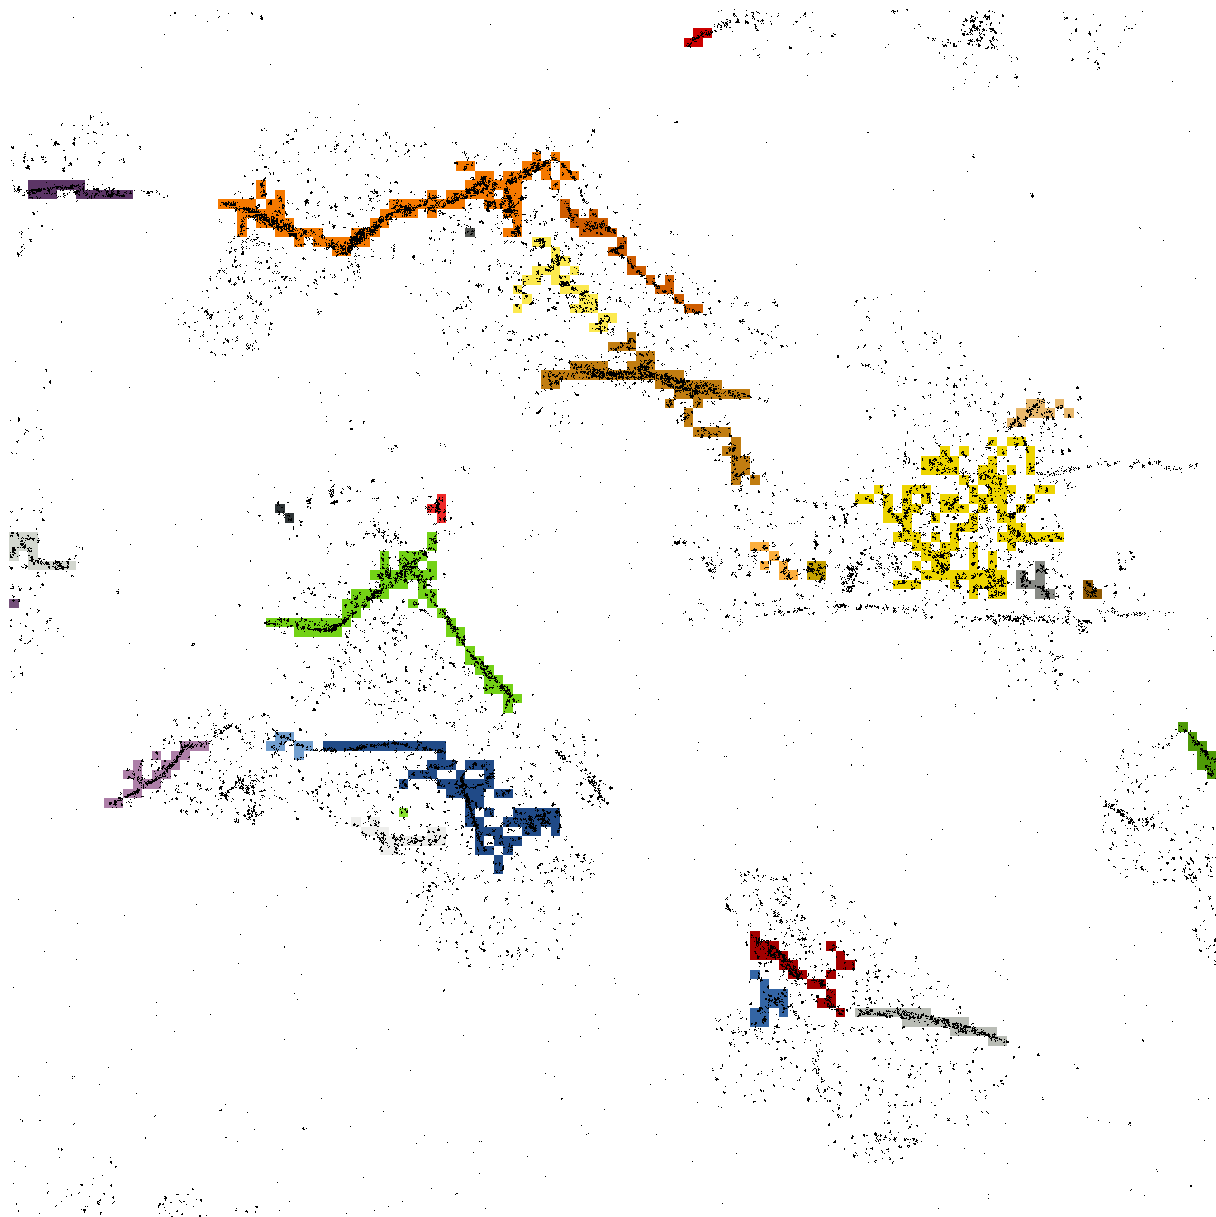
\includegraphics[width=\textwidth]{roundness-long.png}}
		\caption{}\label{fig:roundness-long.png}
	\end{subfigure}%
	\quad
	\begin{subfigure}[b]{4.2cm}
		\fbox{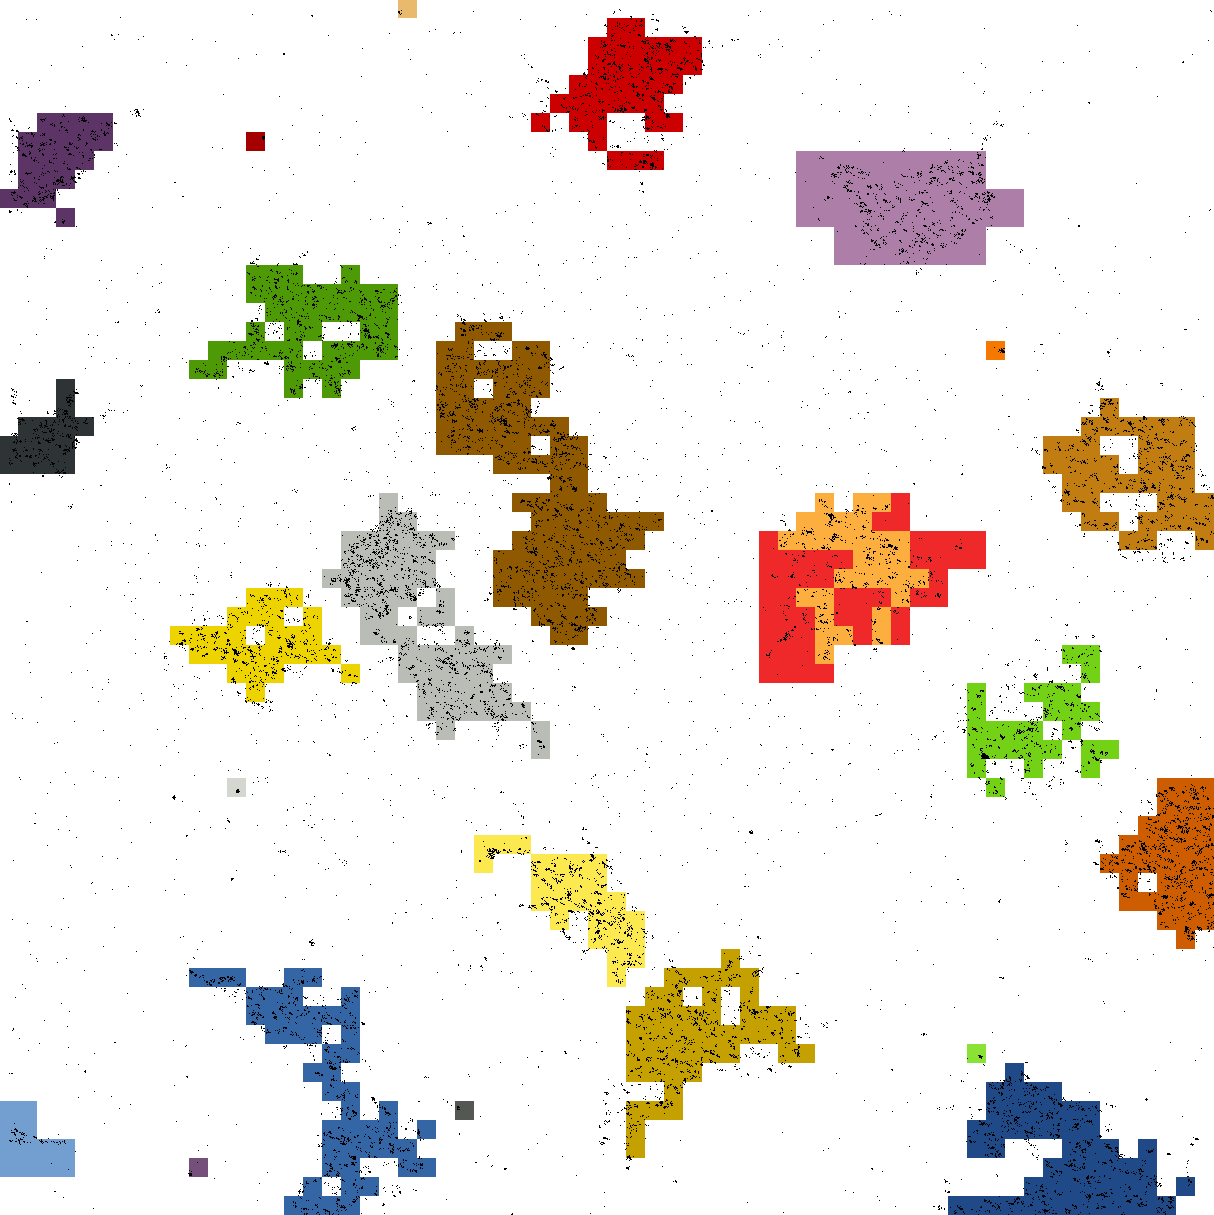
\includegraphics[width=\textwidth]{roundness-round.png}}
		\caption{}
	\end{subfigure}
	% TODO caption
	\caption{}\label{fig:roundness-round.png}
\end{figure}
